\subsection{Conceptos del modelo de negocio}

% Descripcion de la seccion: Esta seccion busca esclarecer los factores relevantes del modelo de negocio sobre el cual se trabajara, para que y como (Descripcion de lo que es un modelo de negocio)

Esta sección esta dedicada a la definición de los conceptos relacionados al modelo de negocio CANVA, información basada del libro \textit{Generación de modelos de negocio de Alexander Osterwalder e Yves Pigneur} \cite{osterwalder2011generacion}.

\subsubsection*{Modelo de Negocio}

El modelo de negocio de una empresa es una herramienta previa al plan de negocio, cuyo objetivo es permitir conocer con claridad el tipo de negocio que se va a crear e introducir en el mercado, a quién va dirigido, cómo se va a vender y cómo se van a conseguir los ingresos. \cite{peiro_2022}


\subsubsection*{Modelo Canvas}
El Modelo CANVAS (The Business Model Canvas) es una metodología, desarrollada por Alexander Osterwalder e Yves Pigneur, la cual se está consolidando como una alternativa real para agregar valor a las ideas de negocio. El modelo Canvas es una herramienta lo suficientemente sencilla como para ser aplicada en cualquier escenario: pequeñas, medianas y grandes empresas, independientemente  de su estrategia de negocio y público objetivo

A continuación en la figura \ref{plantillaModeloCanva} se observa la estructura del Modelo Canva donde se expone el modelo de Negocio

\vspace{2mm}
\begin{minipage}{0.9\textwidth}
\centering
\captionof{figure}[{Modelo Canva}]{ Modelo Canva }
\label{plantillaModeloCanva}
 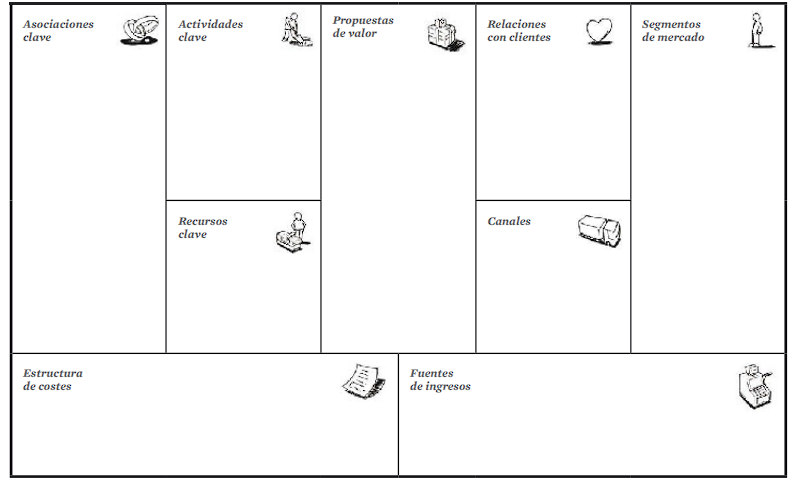
\includegraphics[width=0.7\textwidth]{Images/canva.png}
  %esto es lo nuevo que agregue
\fnote{Nota. \textup{Fuente: Cuente:(Sitio web: ¿Qué es el Modelo Canvas y cómo crear tu propio lienzo o plantilla Business Model Canvas?, según José Facchin, 2020).}}
\end{minipage}

\begin{itemize}
    \item Segmento del Mercado: Son la población objetivo de nuestro modelo de negocio basada en un conocimiento exhaustivo de las necesidades especificas del la misma.
    
    \item Propuesta de Valor: La propuesta de valor es el factor que hace que un cliente se decante por una u otra empresa; su finalidad es solucionar un  problema o satisfacer una necesidad del cliente. Las propuestas  de valor son un conjunto de productos o servicios que satisfacen los requisitos de un segmento de mercado determinado. 
    \item Canales de Distribución : Los canales de comunicación, distribución y venta establecen el contacto entre la empresa y los clientes. Son puntos de contacto con  el cliente que desempeñan un papel primordial en su experiencia. 
    \item Relaciones con el Cliente : Las empresas deben definir el tipo de relación que desean establecer con cada segmento de mercado a través de captación de de clientes, fidelización y/o estimulación de las ventas. 
    \item Fuentes de Ingreso: Hacen referencia al flujo de caja que genera una empresa en los diferentes segmentos de mercado. Existen fuentes de ingreso por transacciones derivadas de pagos puntuales de clientes y/o pagos periódicos realizaos a cambio del suministro de una propuesta de valor o servicio pos-venta de atención al cliente. 
    \item Recursos Clave: Todos los modelos de negocio requieren recursos clave que  permiten a las empresas crear y ofrecer una propuesta de valor, llegar a los mercados, establecer relaciones con segmentos de  mercado y percibir ingresos. Los recursos clave pueden ser físicos, económicos, intelectuales o humanos. Además, la empresa puede tenerlos en propiedad, alquilarlos u obtenerlos de sus socios clave.
    \item Actividades Clave:  Estas actividades son las acciones más importantes que debe implementar una empresa para tener éxito, y al igual que los recursos clave, son necesarias para crear y ofrecer una propuesta de valor, llegar a los mercados, establecer relaciones con clientes y percibir ingresos. Las actividades varían en función del modelo de negocio.
    \item Socios Clave: Las empresas crean alianzas para optimizar sus modelos de negocio, reducir riesgos o adquirir recursos
    \item Estructura de Costos: Describe los principales costes en los que se incurre al trabajar con un modelo de negocio determinado. Tanto la creación y la entrega de valor como el mantenimiento de las relaciones con los clientes o la generación de ingresos tienen un coste.
\end{itemize}
